% \def\course{Math 228}
%
%
%
%
% \title{Discrete Mathematics: An Open Introduction}
% %{\large Course Notes for Math 228 at the University of Northern Colorado}
%
%
%
%
% \author{Oscar Levin}
%
% \date{Fall 2015}
%
% \begin{titlingpage*}



\documentclass[10pt]{article}

\usepackage{url}
\usepackage{xcolor}
\usepackage{tikz}
\usepackage{mdframed}
\usepackage[papersize={7in,10in}, hmargin={.25in, .5in}]{geometry}

\definecolor{bg}{HTML}{00a092}
\pagecolor{bg}

\usepackage[T1]{fontenc}
\usepackage{newpxtext}
\usepackage[vvarbb,cmintegrals,cmbraces,bigdelims]{newpxmath}
\usepackage[scr=rsfso]{mathalfa}% \mathscr is fancier than \mathcal
\linespread{1.04}         % adds more leading (space between lines)
% quantifiers look strange, so change those back to normal:
	\DeclareSymbolFont{mysymbols}{OMS}{cmsy}{b}{n} %note we make the figures bold to better match newpx.  Replace the ``b'' with an ``m'' to undo this.
	%\SetSymbolFont{mysymbols}  {bold}{OMS}{cmsy}{b}{n}
	%\DeclareSymbolFont{myoperators}   {OT1}{cmr} {m}{n}
	%\SetSymbolFont{myoperators}{bold}{OT1}{cmr} {bx}{n}
	\DeclareMathSymbol{\forall}{\mathord}{mysymbols}{"38}
	\DeclareMathSymbol{\exists}{\mathord}{mysymbols}{"39}
	%\DeclareMathSymbol{\pm}{\mathbin}{mysymbols}{"06}
	%\DeclareMathSymbol{+}{\mathbin}{myoperators}{"2B}
	%\DeclareMathSymbol{-}{\mathbin}{mysymbols}{"00}
	%\DeclareMathSymbol{=}{\mathrel}{myoperators}{"3D}


\begin{document}

\pagestyle{empty}





\tikz[remember picture, overlay] \node  at (current page.center){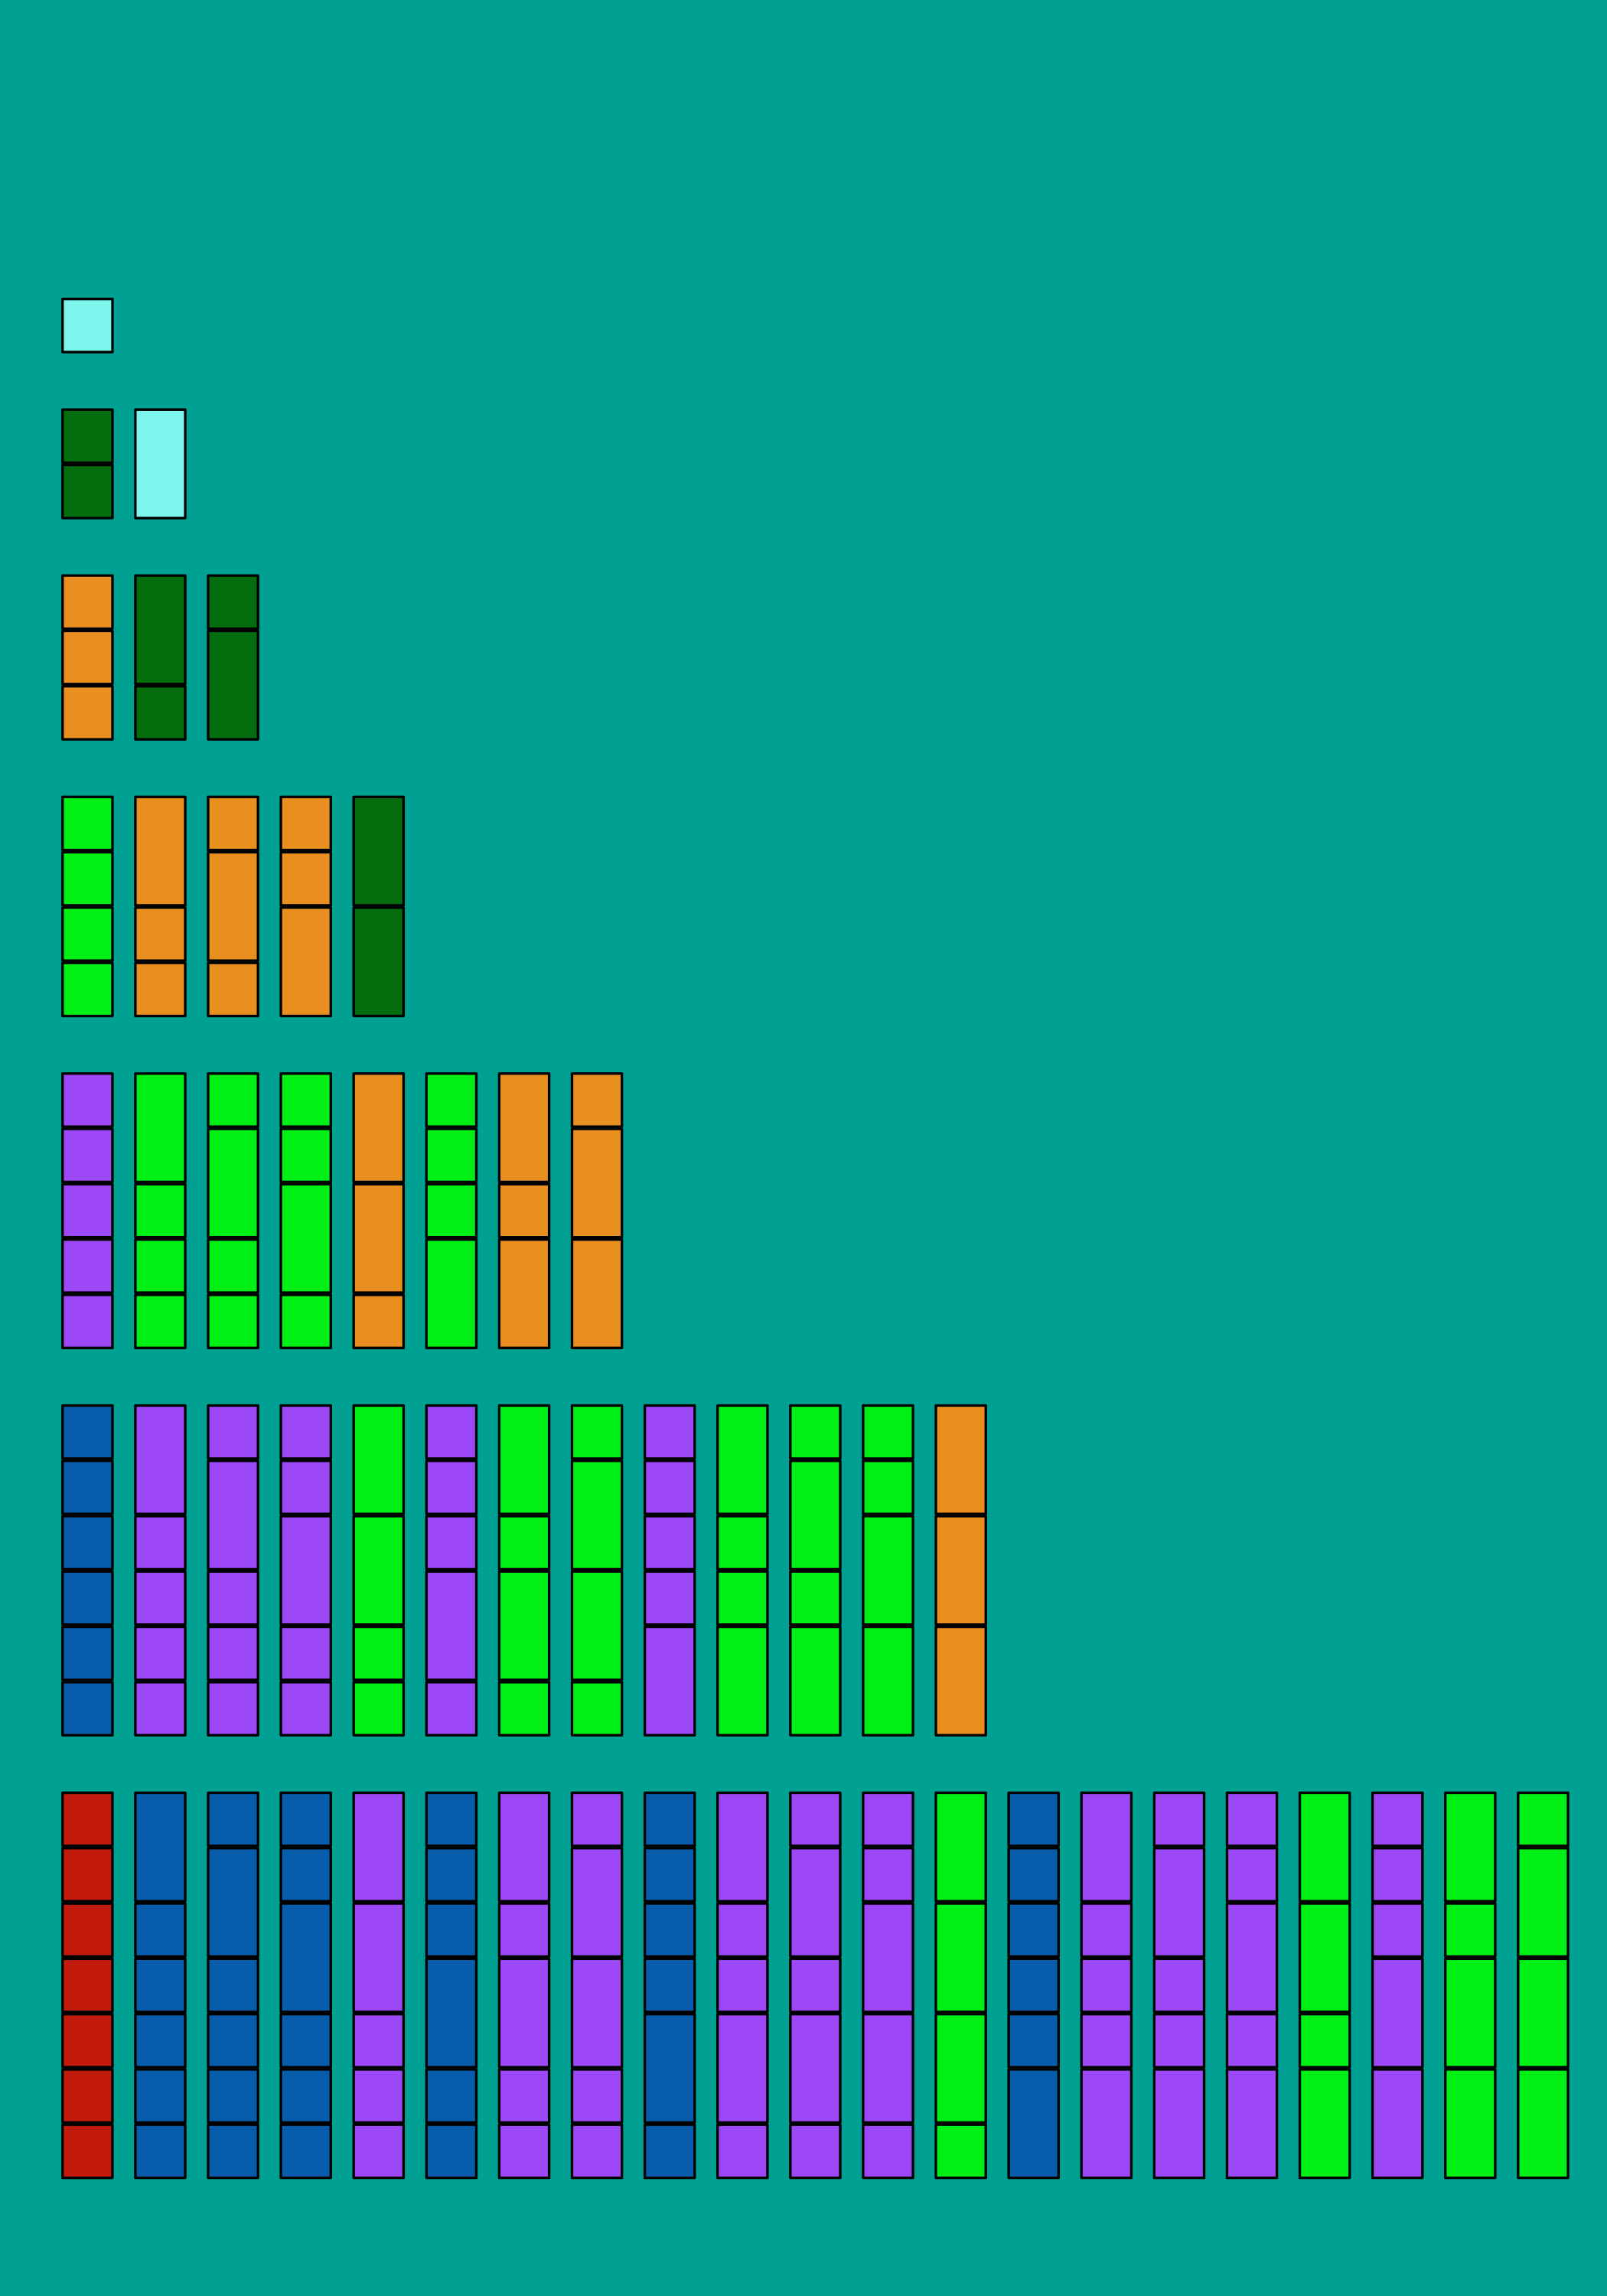
\includegraphics[width=\paperwidth,height=\paperheight]{frontbg}};

\vskip .4in

\begin{flushright}


\resizebox{.6\linewidth}{!}{\scshape Discrete}

\vskip .75em

\resizebox{.8\linewidth}{!}{\scshape Mathematics}

\vskip .6in

\resizebox{.7\linewidth}{!}{\scshape An Open Introduction}

\vskip 1in

\resizebox{.4\linewidth}{!}{\scshape Oscar Levin}

\vskip 1.25in

\resizebox{.25\linewidth}{!}{\scshape 3rd Edition}

\end{flushright}

\clearpage

%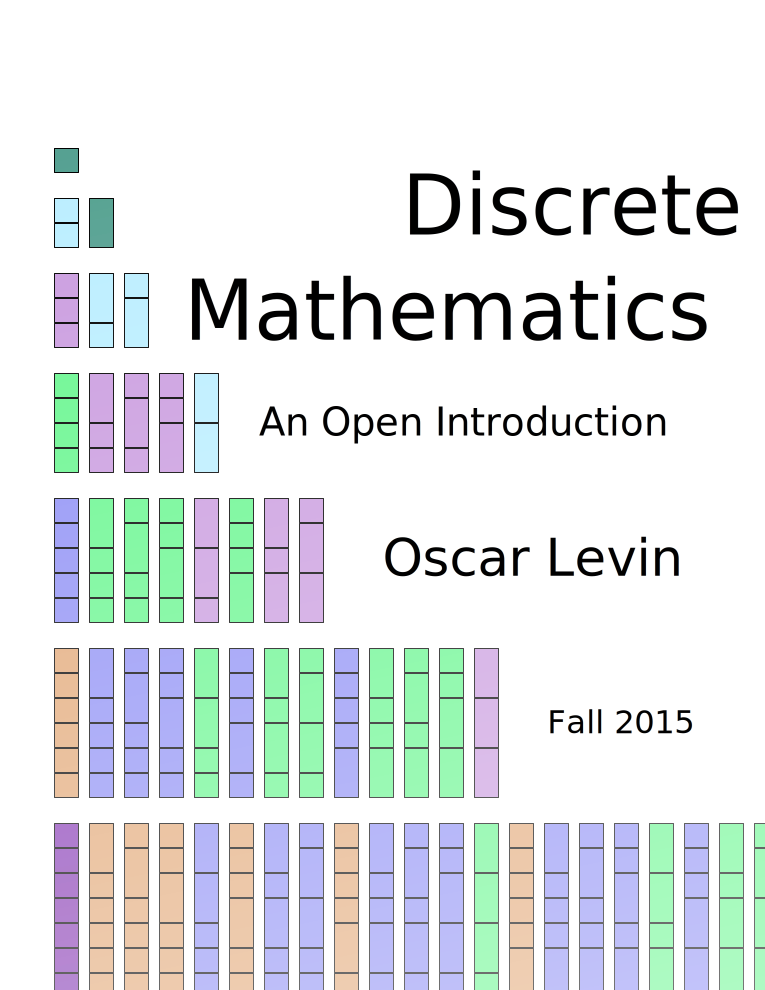
\includepdf[pages=-,pagecommand={\thispagestyle{empty}}]{frontmatter/cover2}
%
%

\end{document}






%\addtocontents{toc}{\protect\thispagestyle{plain}}
